

\chapter*{10 Rekursion}
\addcontentsline{toc}{chapter}{10 Rekursion}
\begin{itemize}[label={}]
    \item \hspace*{-1cm} Definition: eine rekursive Funktion ruft sich selbst auf (evtl. indirekt)
    \item \hspace*{-1cm} Eigenschaften:
    \begin{itemize}
        \item jeder rekursive Aufruf hat seinen eigenen Speicher für alle lokalen Variablen
        \begin{minted}{python}
def f(n):
    r = f(n-1) + 1  # Rekursion
    ...
    return r
        \end{minted}
        \item jede rekursive Funktion muss mindestens einen nicht-rekursiven Zweig haben $\widehat{=}$ Basisfall bzw. Rekursionsabschluss (sonst: Endlosrekursion)
        \item jeder rekursive Aufruf muss nach endlich vielen Rekursionsstufen auf den Basisfall zurückgeführt werden \\
        Anzahl der Stufen bis zum Basisfall $\widehat{=}$ Rekursionstiefe
        \item jede Rekursion kann so umprogrammiert werden, dass stattdessen eine/mehrere Schleifen und ein Stack verwendet werden \\
        $\Rightarrow$ Rekursion und Iteration sind gleich mächtig, welche Algorihmen man damit realisieren kann \\
        in der Praxis: Entscheidung, was effizienter und/oder lesbarer ist
    \end{itemize}
\end{itemize}

Arten der Rekursion:
\begin{itemize}
    \item lineare Rekursion: jeder Ausführungspfad (if: else:) enthält höchstens \emph{einen} rekursiven Aufruf $\Rightarrow$ Rekursionskette
    \item Baumrekursion: es gibt Ausführungspfade mit 2 oder mehr rekursiven Aufrufen \\
    $\Rightarrow$ entsteht verzweigter Rekursionsbaum
\end{itemize}

Beispiel: Fibonacci-Zahlen
0, 1, 1, 2, 3, 5, 8, 13, ...\\
\[f_u = f_{u-1} + f_{u-2}; f_0 = 0, f_1 = 1\]

\textbf{Aufgabe: Alg. zur Berechnung der n-ten Fibonacci-Zahl}\\

\textbf{Variante 1:} naive Implementation der Definition:
\begin{minted}{python}
def fib1(n):
    if n <= 1:
        return n
    else:
        return fib1(n-1) + fib1(n-2)
\end{minted}
Nachteil: Baumrekursion\\
\begin{center}
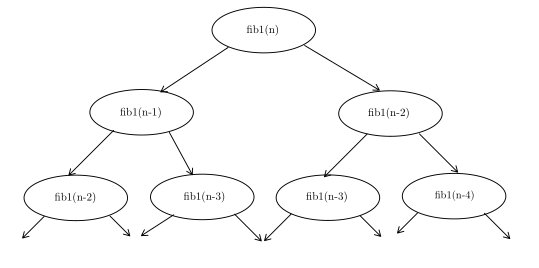
\includegraphics[width=12cm,height=7cm,keepaspectratio]{./Pictures/Fibonacci.png}
\end{center}

Baumtiefe: $\bigO{}(n)$ $\Rightarrow$ Anzahl der Knoten: $\bigO{}(2^n) \widehat{=}$ Komplexität von fib1(n) $\Rightarrow \underline{\text{seeeehr langsam}}$

\textbf{Variante 2:} Umwandlung der Rekursion in Iteration\\

\textbf{Satz:} Jede Rekursion kann mit Hilfe eines Stacks in eine Iteration umgewandelt werden.
\begin{minted}{python}
def fib2(n):
    stack = [n]     #urspruengliches Problem in den Stack legen
    f = 0           #spaeter das Ergebnis
    while len(stack)>0:
        k = stack.pop() #oberstes Teilproblem
        if k <= 1:      #Rekursionsabschluss => Berechnung
            f += k
        else:           #Rekursion => neue Teilprobleme in den Stack
            stack.append(k-1)
            stack.append(k-2)
    return f
\end{minted}

Anzahl der Iterationen = Anzahl rekursive Aufrufe in fib1(n)\\
$\Rightarrow$ Komplexität immer noch $\bigO{}(2^n) \Rightarrow$ Umwandlung in Iteration allein verbessert nie die Komplexität\\

\textbf{Variante 3:} effizienter durch Vermeidung wiederholter Berechnungen der selben Fibonacci-Zahl: \emph{course-of-values-Rekursion} \\

Aufruf für k läuft rekursiv nur von den Aufrufen für k-1, k-2, ..., k-c ab, für konstante c $\Rightarrow$ trifft hier zu mit c = 2

$\Rightarrow$ man kann die Baumrekursion vermeiden, indem man die Zwischenergebnisse so lange speichert, bis sie nicht mehr benötigt werden. \\

Hier: speichere $f_k$, bis $f_{k+2}$ berechnet ist
\begin{minted}{python}
def fib3(n):
    f_n_plus_1, f_n = fib3_impl(n)
    return f_n

def fib3_impl(n):
    if n == 0:
        return 1, 0
    else:
        f_n, f_m_minus_1 = fib3_impl(n-1)
        return f_n + f_n_minus_1, f_n
\end{minted}
entscheidend: Hilfsfunktion ist linear rekursiv $\widehat{=}$ nur 1 rekursiver Aufruf \\
$\Rightarrow$ statt Rekusionsbaum in fib1(n) $\Rightarrow$ Rekusionskette\\
$\Rightarrow$ Komplexität $\bigO{}(N)$, effizienter\\

\textbf{Variante 4:} Umwandeln in Endrekursion $\widehat{=}$ lineare Regression, wo der rekursive Aufruf der letzte Befehl vor dem \emph{return} ist \\

\textbf{Satz:} Jede \emph{Course-of-values-Rekursion} kann in Endrekursion umgeschrieben werden.

\begin{minted}{python}
def fib4(n):
    return fib4_impl(1, 0, n)   #f1, f0, gesuchte Fibonacci-Zahl

def fib4_impl(f_k, f_k_minus_1, counter):
    if counter == 0:            #Rek-Abschluss
        return f_k_minus_1
    else:
        return fib4_impl(f_k + f_k_minus_1, f_k, counter - 1)   #Endrekursion
\end{minted}

\textbf{Variante 5: }Iterative Version ohne Stack\\

\textbf{Satz:} Jede endrekursive Funktion kann ohne Stack in Iteration umgewandelt werden. \\
Idee:
\begin{itemize}
    \item Jeder rekursiveAufruf hat sein eigenes, privates Set lokaler Variablen
    \item ist der rekursive Aufruf der letzte Befehl, werden lokale Variablen \emph{danach} nicht mehr benötigt
\end{itemize}
$\Rightarrow$ wir können die lokalen Variablen für den rekursiven Aufruf recyclen $\widehat{=}$ Überschreiben von Variablen in jeder Schleifeniteration \\

$\rightarrow$ Manche Programmiersprachen (LISP, SCHEME) machen diese Optimierung automatisch\\

\begin{minted}{python}
def fib5(n):
    f_k, f_k_minus_1 = 1, 0
    while n > 0:
        f_k, f_k_minus_1 = f_k + f_k_minus_1, f_k
        n -= 1
    return f_k_minus_1
\end{minted}
n Iterationen $\Rightarrow$ $\bigO{}(n)$\\

\textbf{Variante 6:} (Hausaufgabe) Komplexität $\bigO{}(log N)$ \\

\section*{10.1 Umwandlung von Rekursion in Iteration}
\addcontentsline{toc}{section}{10.1 Umwandlung Rekursion in Iteration}
\textbf{Beispiel für Umwandlung von Rekursion in Iteration mit Stacks}
\begin{minted}{python}
def tree_sort(node, a):     #Aufgabe: geg.Suchbaum, Schluessel in aufsteigender Reihenfolge auslesen und in Array a kopieren
    if node is None: return     #Rekursionsabschluss
    tree_sort(node.left, a)     # kleine Schluessel
    a.append(node.key)          # "mittleren Schluessel" einfuegen
    tree_sort(node.right, a)    #grosse Schluessel
\end{minted}
in-order-trav...

\begin{minted}{python}
def tree_sort_iterative(node, a):
    stack = []
    traverse_left(node, stack)
    while len(stack) > 0:
        current = stack.pop()
        a.append(current.key)
        traverse_left(current.right, stack)
\end{minted}
\begin{minted}{python}
def traverse_left(node, stack):
    while node is not None:
        stack.append(node)
        node = node.left
\end{minted}

Komplexität: $\bigO{}(2^P) = \bigO{}(2^{log N}) = \bigO{}(N)$ falls Baum balanciert \\

\section*{10.2 Komplexitätsberechnung rekursiver Algorithmen}
\addcontentsline{toc}{section}{10.2 Komplexitätsberechnung rekursiver Algorithmen}
\[ T(n) = \underbrace{a_1 * T\left(\frac{N}{b_1}\right)}_{\text{Aufwand für $a_1$ rekursive Teilprobleme der Größe N/$b_1$}} + \cdots + \underbrace{a_n* T\left(\frac{N}{b_n}\right)}_{a_n \text{Teilprobleme der Größe} \frac{N}{b_n}} + \underbrace{f(N)}_{\text{Aufwand der aktuellen Fkt}}\]

fib1(n) : 1 Aufruf(n-1), 1 Aufruf(n-2) $\Rightarrow$ 2 Aufrufe $\bigO{}(N)$ \\
\hspace*{5cm} $n_1 = 2, b_1 = 1, k = 1$ \\
Ausrechnen durch
\begin{itemize}
    \item Substitutionsmethode (\glqq händisch\grqq) $\Rightarrow$ später
\end{itemize}
    \subsection*{10.2.1 Mastertheorem}
    \begin{itemize}
    \item \textbf{Mastertheorem} (einsetzen): $T(n) = a* T\left(\frac{N}{b}\right) + f(n)$
    \addcontentsline{toc}{subsection}{10.2.1 Mastertheorem}
    \begin{itemize}[label={}]
        \item Definiere Rekursionsexponent: $\rho = log_b(a)$
        \item \textbf{Fall 1}: $f(N)$ sehr effizient: $f(N) \in \bigO{}(N^{\rho-\epsilon}), \epsilon > 0$ \\
        $\Rightarrow$ $T(N) \in \Theta(N^\rho)$Rekursion dominiert
        \item \textbf{Fall 2}: $f(N)$ so effizient wie Rekursion: $f(N) \in \Theta(N^\rho)$ \\
        $\Rightarrow T(N) \in \Theta(N^\rho * logN) \Rightarrow$ Rekursion und f(N) tragen bei
        \item \textbf{Fall 3}: $f(N)$ nicht so effizient: $f(N) \in \Omega(N^{\rho + \epsilon}), \epsilon > 0$ \\
        \hspace*{5cm} $a f\left(\frac{N}{b}\right) \leq c* f(N)$ mit $c < 1$ \\
        $\Rightarrow T(N) \in \Theta(f(N)) \Rightarrow f(N)$ dominiert
    \end{itemize}
    \item \textbf{Beispiel} Merge Sort: $T(N)\ =\ \underbrace{2 T \ \left(\frac{N}{2}\right)}\hspace*{0.7cm} +\hspace*{0.7cm} \underbrace{\Theta\ (N)}$\\
    \begin{tabular}{L{4cm} L{3cm} L{3cm}}
        $a=2, b=2$ & rekursive Aufrufe für linke und rechte Hälfte & Zusammenfügen der sortierten Hälften\\
    \end{tabular}\\
    \hspace*{1cm} $\rho = log_b(a) \ = \ log_2(2) \ = \ 1 \ \Rightarrow \ f(N)\ \in \ \Theta(N^2) \ = \ \Theta(N)$\\
    $\Rightarrow$ Fall 2  \hspace*{1cm} $T(N)\  \in\  \Theta(N^{\rho}\ log\ N)\ =\ \boxed{\Theta(N\ log(N))}$ wie bekannt
\end{itemize}

    \subsection*{10.2.2 Substitutionsmethode}
    \addcontentsline{toc}{subsection}{10.2.2 Substitutionsmethode}
    \subsubsection*{Händisches Berechnen mittels Substitutionsmethode}
    \begin{itemize}
        \item \textbf{Beispiel}: Merge Sort, wo wir in zwei ungleich große Teilprobleme aufspalten \\
        \[ T(N)\ =\ T\left(\frac{N}{3}\right)\ +\ T\left(\frac{2N}{3}\right)\ +\ \Theta(N)\]
        zeige jetzt: ungleiche Aufteilung ändert nicht die Komplexität
        \item \textbf{Rekursionsbaum}:\\
        \begin{center}
        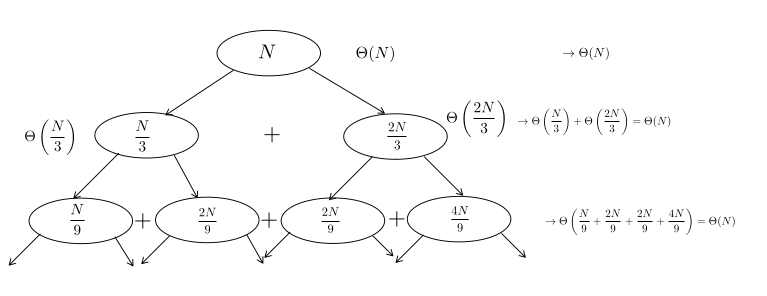
\includegraphics[width=15cm,height=8cm,keepaspectratio]{./Pictures/Substitutionsmethode.png}
        \end{center}
        Berechnen des Aufwands der eigentlichen Berechnung in jedem Knoten ohne Rekursion\\
        $\Rightarrow$ pro Ebene: $\Theta(N) \ \Rightarrow$ Gesamtaufwand $\Theta(N*D)$ $D\ \dots$ Tiefe des Baums \\
        Rekursion endet, wenn Knoten nur 1 Element enthält: $\left(\frac{2}{3}\right)^D * N = 1$\\
        \hspace*{1cm} $\Rightarrow\ D\ =\ log_{3/2}(N)\ = \ \bigO{}(log\ N)$
        \item Vermutung: $T(N)\ \in\ \bigO{}(log_{3/2}(N)\ *\ c*N)\ =\ \bigO{}\ (log\ N\ *\ N)$\\
        falls die Vermutung gilt, gilt für großes N:
        \[ T(N)\ \leq\ d\ *\ N\ *\ \underbrace{log_2(N)}_{ld}\ \text{Definition der O-Notation mit passender Konstante d}\]
        Einsetzen in Rekursionsformel
        \[ T(N)\ =\ T\left(\frac{N}{3}\right)\ +\ T\left(\frac{2N}{3}\right)\ +\ c*N \ \leq d \frac{N}{3} ld\left(\frac{N}{3}\right)\ + d\frac{2N}{3} ld\left(\frac{2N}{3}\right)\ +\ c*N\]
        \[ \leq d*\frac{N}{3} ld(N)\ -\ d\frac{N}{3} ld(3)\ +\d*\frac{2N}{3} ld(N)\ -\ d\frac{2N}{3} \underbrace{ld(2)}_{=1}\ - d\frac{2N}{3} ld(3)\ +\ c*N \]
        \[ d\ N\ ld(N)\ \underbrace{-\ d\ N\ \left(ld(3)\ -\ \frac{2}{3}\ \right)\ +\ c*N}_{\text{sollte} \leq 0\text{sein}} - d\ \not N\  \left(ld(3)\ - \ \frac{2}{3}\ \right)\ +\ c*\ \not N\ \leq\ 0\]
        mit:
        \hspace*{1cm} $d\ \left(\ ld(3)\ -\ \frac{2}{3}\right)\ +\ c* \not N \leq 0$ und $d\ \left(\ ld(3)\ -\ \frac{2}{3}\right)\ \geq c$ immer erreichbar, weil beliebig groß gewählt werden darf
        \[ \leq d\ N\ ld(N) \Rightarrow \text{Vermutung bestätigt}\]
        $\Rightarrow T(N)\ \in\ \bigO{}(N\ log\ N)\  \text{w. z. b. w.}$
    \end{itemize}

%TODO fehlt...

